\documentclass[12pt]{article}

\usepackage[margin=1cm]{geometry}
\usepackage{graphicx}
\usepackage{amsmath}
\usepackage{xcolor}
\usepackage{pagecolor}
\usepackage{mathtools}
\usepackage[font={color=white,bf}]{caption}
\usepackage{float}
\usepackage{tikz}
\usetikzlibrary{positioning, calc}
\usepackage{tkz-euclide}
\usepackage{subcaption}
\usepackage{nicefrac}

\renewcommand{\maketitle}{
	\begin{center}
		\Large{
			\textbf{Classical Mechanics}

		Lecture Notes
		}
		\vspace{5pt}
	
		\normalsize{
			Tyler Forshaw
	
			\today
		}
		\vspace{15pt}
	\end{center}
}

\begin{document}
\color{white}
\pagecolor{black!85!}
\maketitle

\section{Dimensional Analysis}
Hypothesis: Pressure is (linear) momentum flux.

\begin{alignat*}{2}
	\text{Pressure}      & = \frac{F}{A} = \frac{ma}{A}
	                     &                              & = \frac{[M][L][T]^{-2}}{[L]^2} = [M][L]^{-1}[T]^{-2}    \\
	\text{Momentum Flux} & = \frac{mv}{At}
	                     &                              & = \frac{[M][L][T]^{-1}}{[L]^2[T]} = [M][L]^{-1}[T]^{-2}
\end{alignat*}

\subsection{Planck Units}
\begin{description}
	\item[$\hbar$] --- Planck's constant ($\hbar = \frac{h}{2\pi}$)
	\item[$G$] --- Gravitational constant
	\item[$c$] --- Speed of light
\end{description}

\section{Is the LHC a \emph{Big bang machine}}

\subsection{Performing dimensional analysis on the \emph{planck time}}
\begin{flalign*}
	T_p & = \hbar^\alpha G^\beta c^\gamma                                                                                          & \\
	[T] & = \left(\frac{[M][L]^2}{[T]}\right)^\alpha \left(\frac{[L]^3}{[M][T]^2}\right)^\beta \left(\frac{[L]}{[T]}\right)^\gamma &
\end{flalign*}
From this analysis, you can derive that the correct equation is: $T_p = \sqrt{\frac{\hbar G}{c^5}}$

\begin{align*}
	E_p & = h^\alpha G^\beta c^\gamma    & \text{Plank energy }                               \\
	1   & = \alpha - \beta               & 2                    & = 2\alpha + 3\beta + \gamma \\
	2   & = -\alpha -2\beta + \gamma                                                          \\
	\phantom{=}                                                                               \\
	    & \implies \sqrt{\frac{hc^5}{G}}                                                      \\
	    & \approx 10^9 ~J = 10^{19} ~GeV
\end{align*}

\begin{flalign*}
	 & \text{Energy in the very early universe}          & E_{\text{BB}}  & \approx 10^{19} ~GeV & \\
	 & \text{While the typical energy in the \emph{LHC}} & E_{\text{LHC}} & \approx 10^{4} ~GeV  &
\end{flalign*}

\subsection{Basic wind power calculations}
\begin{align*}
	E_k           & = \frac{1}{2}mv^2                       &
	P             & = \frac{E_k}{t}
	              &                                         & \text{Across the swept area of the blades} & \phantom{=}                                                                           \\
	\phantom{=}                                                                                                                                                                                  \\
	m             & = \rho Avt                              &                                            &              &  & \text{Cylinder of air with cross section } A \text{ and length } vt \\
	\phantom{=}                                                                                                                                                                                  \\
	\phantom{=}                                                                                                                                                                                  \\
	E_k           & \approx \rho Avt \, v^2
	              & P_k                                     & \approx \rho A \, v^3                                                                                                              \\
	              & = \frac{1}{2} \rho At \, v^3                                                                                                                                                 \\
	\phantom{=}                                                                                                                                                                                  \\
	\phantom{=}                                                                                                                                                                                  \\
	S             & = n^2 t^2                               &                                            &              &  & \text{Measure surface in number of wind turbine radii}              \\
	\phantom{=}                                                                                                                                                                                  \\
	\phantom{=}                                                                                                                                                                                  \\
	\frac{P_k}{S} & = \frac{\rho Av^3}{S}                   &                                            &              &  & \text{Power available per unit surface}                             \\
	              & = \rho \frac{\pi t^2 v^3}{n^2 t^2}                                                                                                                                           \\
	              & = \frac{\rho \pi v^3}{n^2}                                                                                                                                                   \\
	\phantom{=}                                                                                                                                                                                  \\
	\phantom{=}                                                                                                                                                                                  \\
	\rho          & \approx 1 ~kg \, m^{-1}
	              & v                                       & \approx 5 ~ms^{-1}                                                                                                                 \\
	n             & = 10                                    &                                            &              &  & \text{Free variable } n                                             \\
	\phantom{=}                                                                                                                                                                                  \\
	\phantom{=}                                                                                                                                                                                  \\
	\frac{P_k}{S} & = \frac{\rho \pi v^3}{n^2}              &
	\frac{P_k}{S} & \approx \frac{1 \cdot 3 \cdot 100}{100}                                                                                                                                      \\
	              &                                         &                                            & = 3 ~Wm^{-2}                                                                          \\
\end{align*}
\begin{align*}
	\text{UK pop}               & \approx 70 ~\text{Million}                                                  &  & \text{UK surface area} \approx 2.5 \times 10^{11} ~m^2 \\
	\text{UK avg power}         & \approx 125 ~kWh/\text{person}/\text{day}                                                                                               \\
	                            & \approx \frac{(125 \times 10^3) \times (3.6 \times 10^3)}{8.64 \times 10^4}                                                             \\
	                            & = \frac{125 \times 10^2 \times 3.6}{8.64}                                                                                               \\
	                            & \approx 6.25 \times 10^3 ~kW/\text{person}                                                                                              \\
	\phantom{=}                                                                                                                                                           \\
	\phantom{=}                                                                                                                                                           \\
	\implies (6.25 \times 10^3) & \times (70 \times 10^6) = 4.375 \times 10^{11} ~W
\end{align*}

\section{Vectors}
\begin{description}
	\item[Mangitude] --- $\displaystyle \left|\overrightarrow{a}\right|$
	\item[Unit vector] --- $\displaystyle \frac{\overrightarrow{a}}{\left|\overrightarrow{a}\right|} = \hat{a}$
	\item[Dot product] --- $\displaystyle \overrightarrow{a} \cdot \overrightarrow{b} = |\overrightarrow{a}| |\overrightarrow{b}| \cos{\theta}$
\end{description}

\begin{align*}
	\overrightarrow{a}                      & = a_x \hat{e}_x + a_y \hat{e}_y + a_z \hat{e}_z                         \\
	\overrightarrow{a} + \overrightarrow{b} & = \overrightarrow{c}                                                    \\
	\overrightarrow{a} - \overrightarrow{b} & = \overrightarrow{d}                                                    \\
	\overrightarrow{a} + \overrightarrow{b} & = (a_x + b_x) \hat{e}_x + (a_y + b_y) \hat{e}_y + (a_z + b_z) \hat{e}_z
\end{align*}

Project the component of $a$ along the $\hat{e}$ direction
\begin{align*}
	\overrightarrow{b}                             & = \hat{e}                                                                        & |\hat{e}| & = 1 \\
	\overrightarrow{a} \cdot \hat{e}               & = |\overrightarrow{a}| \cos{\theta}                                                                \\
	\phantom{=}                                                                                                                                         \\
	\overrightarrow{a} \times \overrightarrow{b}   & = \overrightarrow{c}                                                                               \\
	\overrightarrow{c} \text{ is perpendicular to} & \text{ the plane containing } \overrightarrow{a} \text{ and } \overrightarrow{b}                   \\
	|\overrightarrow{c}|                           & = |\overrightarrow{a}| |\overrightarrow{b}| \sin{\theta}
\end{align*}

\section{Kinematics}
A point moving through a curved trajectory

\begin{align*}
	\overrightarrow{R}(t):                 & \text{Position}                                                                                                 \\
	\frac{d \overrightarrow{R}(t)}{dt}     & = \overrightarrow{v}(t)                                                                                         \\
	\lim_{\delta t \to 0} \frac{\delta \overrightarrow{R}}{\delta t}                                                                                         \\
	\phantom{=}                                                                                                                                              \\
	\frac{d^2 \overrightarrow{R}(t)}{dt^2} & = \frac{d \overrightarrow{v}(t)}{dt} = \overrightarrow{a}(t)                                                    \\
	\lim_{\delta t \to 0} \frac{\delta^2 \overrightarrow{R}}{\delta t^2}                                                                                     \\
	\phantom{=}                                                                                                                                              \\
	\overrightarrow{R}(t)                  & = R_x(t) \hat{e}_x + R_y(t) \hat{e}_y + R_z(t) \hat{e}_z                                                        \\
	\phantom{=}                                                                                                                                              \\
	\overrightarrow{v}(t)                  & = \frac{dR}{dt} = \frac{d R_x(t)}{dt} \hat{e}_x + \frac{d R_y(t)}{dt} \hat{e}_y + \frac{d R_z(t)}{dt} \hat{e}_z \\
\end{align*}

\section{Time and Length Contraction}
\subsection{Time dilation}
\begin{align*}
	f_\text{obs}                                                           & = \sqrt{\frac{1 + \frac{u}{c}}{1 - \frac{u}{c}}} f_\text{rest}                                     \\
	\sqrt{\frac{1 + \frac{1}{2} \frac{u}{c}}{1 - \frac{1}{2} \frac{u}{c}}} & = \sqrt{\frac{1+\frac{1}{2}}{1 - \frac{1}{2}}} = \sqrt{3}      &  & \text{When } u = \frac{1}{2} c \\
	\phantom{=}                                                                                                                                                                 \\
	f_\text{jack}                                                          & = \sqrt{3} f_\text{linda}                                                                          \\
	\lambda_\text{linda}                                                   & = 680 ~nm                                                                                          \\
	\frac{c}{\lambda_\text{jack}}                                          & = \sqrt{3} \frac{c}{\lambda_\text{linda}}                                                          \\
	\phantom{=}                                                                                                                                                                 \\
	\phantom{=}                                                                                                                                                                 \\
	\lambda_\text{jack}                                                    & = \frac{680 ~nm}{\sqrt{3}} \approx 392 ~nm
\end{align*}

\begin{align*}
	u                     & = \frac{1}{2} c                                                                                           &  & \text{Jack moving towards Linda} \\
	\gamma                & = \frac{1}{\sqrt{1 - \frac{u^2}{c^2}}}                                                                                                          \\
	                      & = \frac{1}{\sqrt{1 - \left(\frac{1}{2}\right)^2}} = \frac{1}{\sqrt{1 - \frac{1}{4}}} = \frac{2}{\sqrt{3}}                                       \\
	\phantom{=}                                                                                                                                                             \\
	\Delta t_\text{Jack}  & = 3 ~ \text{months}                                                                                       &  & \Delta t_\text{Linda} = \  ?     \\
	\phantom{=}                                                                                                                                                             \\
	\Delta t_\text{obs}   & = \gamma \Delta t_\text{rest}                                                                                                                   \\
	\Delta t_\text{Linda} & = \frac{2}{\sqrt{3}} \Delta t_\text{Jack}                                                                                                       \\
	                      & = \frac{2}{\sqrt{3}} \times 3 ~ \text{months}                                                                                                   \\
\end{align*}

\subsection{Length Contraction}
\begin{align*}
	u                        & = 0.995 c ~ms^{-1}                                                                              \\
	\phantom{=}                                                                                                                \\
	\gamma                   & = \frac{1}{\sqrt{1 - \frac{(0.995c)^2}{c^2}}}                                                   \\
	                         & = \frac{1}{\sqrt{1 - 0.995^2}}                                                                  \\
	                         & \approx 10                                                                                      \\
	\phantom{=}                                                                                                                \\
	\text{Elizabeth's frame} &                                                                                                 \\
	D_\text{ship}            & = 30 ~ km \, s^{-1}                                                                             \\
	D_E                      & = \frac{1}{\gamma} D_\text{ship}              & \gamma  & = 10                                  \\
	                         & = \frac{1}{10} D_\text{ship}                                                                    \\
	                         & = \frac{30}{10} = 3 ~ km \, s^{-1}                                                              \\
	\phantom{=}                                                                                                                \\
	\tau_\text{Activation}   & = 10^{-5} ~s                                  & u       & = 0.995 c ~ms^{-1}                    \\
	\text{The ship's frame}  &                                                                                                 \\
	\gamma                   & = 10                                                                                            \\
	t_\text{obs}             & = \gamma t_\text{rest}                                                                          \\
	t_\text{ship}            & = \gamma t_{(E)}                              & t_{(E)} & = \tau_\text{Activation} = 10^{-5} ~s \\
	                         & = 10 \cdot 10^{-5} ~ s                                                                          \\
	                         & = 10^{-4} ~ s                                                                                   \\
	t_\text{ship}            & = 30 ~km                                                                                        \\
\end{align*}

\section{Dynamics}
\begin{description}
	\item[Newton's Laws] --- Forces, Work done by force
\end{description}

\begin{enumerate}
	\item If no force active upon a boy $\implies u$
	\item $\overrightarrow{F} = \underbrace{m}_{\hidewidth \text{Intertial mass}\hidewidth} \overrightarrow{a}$
	\item $\overrightarrow{F_{A \to B}} = -\overrightarrow{F_{B \to A}}$
\end{enumerate}

\subsection{Principle of superposition}
\begin{align*}
	\overrightarrow{F_\text{total}} & = \overrightarrow{F_1} + \overrightarrow{F_2} + \overrightarrow{F_3} + \hdots \\
	                                & = \displaystyle\sum_{i=1}^N \overrightarrow{F_k} = m \overrightarrow{a}       \\
	\overrightarrow{a}              & = \frac{1}{m} \displaystyle\sum_k^N \overrightarrow{F_k}
\end{align*}

\subsection{Dynamics Examples}
\subsubsection{Weight}
\begin{figure}[h!]
	\begin{subfigure}{.45\textwidth}
		\begin{center}
			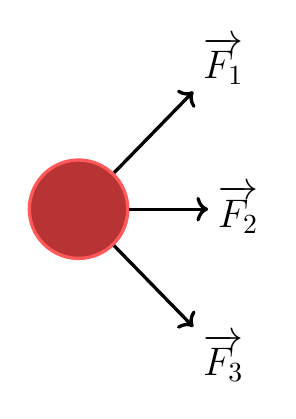
\begin{tikzpicture}[
					PhysNode/.style={circle, draw=red!65, fill=red!65!black!80, very thick, minimum size=1.25cm}]

				% Nodes
				\node[PhysNode] (ForceNode) {};
				\node[font=\Large] (F1) [above right=of ForceNode]{$\overrightarrow{F_1}$};
				\node[font=\Large] (F2) [right=of ForceNode] {$\overrightarrow{F_2}$};
				\node[font=\Large] (F3) [below right=of ForceNode] {$\overrightarrow{F_3}$};

				% Lines
				\draw[very thick, ->] (ForceNode) to (F1);
				\draw[very thick, ->] (ForceNode) to (F2);
				\draw[very thick, ->] (ForceNode) to (F3);
			\end{tikzpicture}
		\end{center}
		\caption{Force diagram}
	\end{subfigure}
	\begin{subfigure}{.45\textwidth}
		\begin{center}
			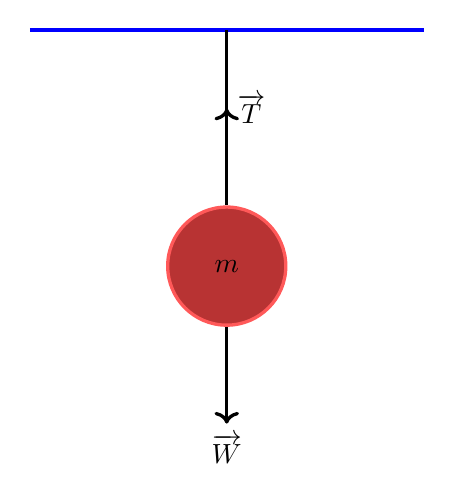
\begin{tikzpicture}[
					PhysNode/.style={circle, draw=red!65, fill=red!65!black!80, very thick, minimum size=1.5cm}]

				\node[PhysNode] (Mass) {$m$};

				\draw[ultra thick, blue] ($(Mass) - (2.5cm, -3cm)$) -- ($(Mass) + (2.5cm, 3cm)$);
				\draw[very thick] ($(Mass) + (0cm, 3cm)$) -- (Mass);
				\draw[very thick, <-] ($(Mass) + (0cm, 2cm)$) -- (Mass) ($(Mass) + (0cm, 2cm)$) node[right=0] () {$\overrightarrow{T}$};
				\draw[very thick, ->] (Mass) -- ($(Mass) - (0cm, 2cm)$) node[below=0cm] () {$\overrightarrow{W}$};
			\end{tikzpicture}
		\end{center}
		\caption{Tension diagram}
	\end{subfigure}
\end{figure}

\begin{align*}
	\text{Resolving } \uparrow \qquad \quad &     & \text{Resolving } \downarrow \qquad \quad &     \\
	T - W                                   & = 0 & W - T                                     & = 0 \\
	T                                       & = W & T                                         & = W \\
\end{align*}

\subsubsection{Friction}
\begin{figure}[H]
	\begin{center}
		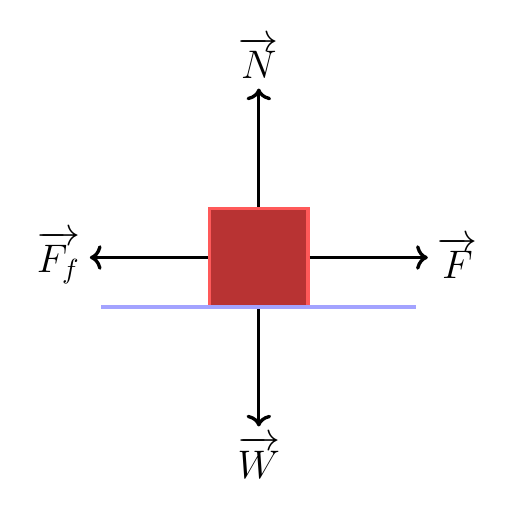
\begin{tikzpicture}[
				PhysNode/.style={rectangle, draw=red!65, fill=red!65!black!80, very thick, minimum size=1.25cm}]

			% Nodes
			\node[PhysNode] (ForceNode) {};

			\node[font=\Large] (N) [above=1.5cm of ForceNode]{$\overrightarrow{N}$};
			\node[font=\Large] (W) [below=1.5cm of ForceNode]{$\overrightarrow{W}$};
			\node[font=\Large] (Ff) [left=1.5cm of ForceNode]{$\overrightarrow{F_f}$};
			\node[font=\Large] (F) [right=1.5cm of ForceNode]{$\overrightarrow{F}$};

			% Lines
			\draw[very thick, ->] (ForceNode) to (N);
			\draw[very thick, ->] (ForceNode) to (W);
			\draw[very thick, ->] (ForceNode) to (Ff);
			\draw[very thick, ->] (ForceNode) to (F);

			\draw[ultra thick, blue!60!white!60] (-2cm, -0.625cm) -- (2cm, -0.625cm);

			\coordinate (P) at (1, 0);
		\end{tikzpicture}
	\end{center}
	\caption{Friction diagram}
\end{figure}

\begin{align*}
	|\overrightarrow{F_f}| = \mu |\overrightarrow{N}| \\
	\phantom{=}                                       \\
	\begin{rcases}
		\text{Static: }  & \mu_s \\
		\text{Kinetic: } & \mu_k \\
	\end{rcases}
	\mu_s > \mu_k
\end{align*}

\subsubsection{Tension}
\begin{figure}[H]
	\begin{center}
		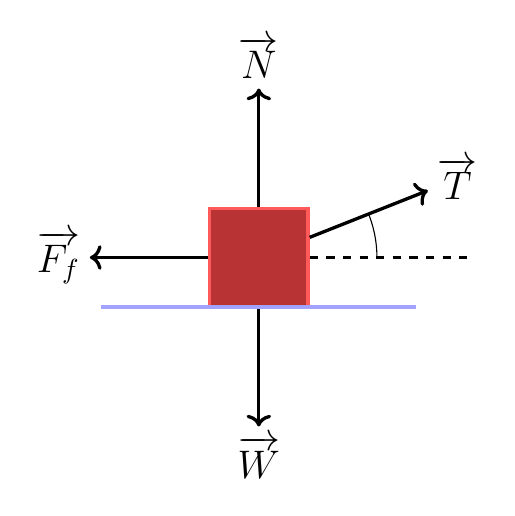
\begin{tikzpicture}[
				PhysNode/.style={rectangle, draw=red!65, fill=red!65!black!80, very thick, minimum size=1.25cm}]

			% Nodes
			\node[PhysNode] (ForceNode) {};

			\node[font=\Large] (N) [above=1.5cm of ForceNode]{$\overrightarrow{N}$};
			\node[font=\Large] (W) [below=1.5cm of ForceNode]{$\overrightarrow{W}$};
			\node[font=\Large] (Ff) [left=1.5cm of ForceNode]{$\overrightarrow{F_f}$};
			\node[font=\Large] (T) [right=1.5cm of ForceNode, yshift=1cm]{$\overrightarrow{T}$};

			% Lines
			\draw[very thick, ->] (ForceNode) to (N);
			\draw[very thick, ->] (ForceNode) to (W);
			\draw[very thick, ->] (ForceNode) to (Ff);
			\draw[very thick, ->] (ForceNode) to (T);

			\draw[very thick, dashed] (ForceNode.east) to ++(2cm,0);

			\draw[ultra thick, blue!60!white!60] (-2cm, -0.625cm) -- (2cm, -0.625cm);

			\coordinate (P) at (1, 0);

			\tkzMarkAngle[size=1.5cm](P,ForceNode,T)
			\tkzLabelAngle[pos=3.2pt](P,ForceNode,T){\color{white}$\theta^\circ$}
		\end{tikzpicture}
	\end{center}
	\caption{Tension diagram}
\end{figure}

What is the angle $\theta$ which minimises $F$

\begin{itemize}
	\item{Moving with constant velocity}
	\item{Ignore static friction}
	\item{$\mu_k = \mu$}
\end{itemize}
\begin{align*}
	v \equiv v_x = \text{const}                                                                                                                                                       \\
	a \equiv a_x = \frac{dv}{dx} = 0                                                                                                                                                  \\
	\phantom{=}                                                                                                                                                                       \\
	\text{Perpendicular component } z                  &
	                                                   & \text{Parallel component } x                     &                                                                           \\
	N - mg + \overrightarrow{F} \sin{\theta}           & = 0
	                                                   & \overrightarrow{F} \cos{\theta} - \mu N          & = m \overbrace{\overrightarrow{a}}^0 = 0                                  \\
	                                                   &                                                  & F \cos{\theta}                           & = \mu N                        \\
	                                                   &                                                  & N                                        & = \frac{1}{\mu} F \cos{\theta} \\
	\phantom{=}                                                                                                                                                                       \\
	\phantom{=}                                                                                                                                                                       \\
	\frac{1}{\mu} F \cos{\theta} - mg + F \sin{\theta} & = 0                                                                                                                          \\
	F \cos{\theta} - \mu mg + \mu F \sin{\theta}       & = 0                                                                                                                          \\
	F(\cos{\theta} + \mu \sin{\theta})                 & = \mu mg                                                                                                                     \\
	\phantom{=}                                                                                                                                                                       \\
	F                                                  & = \frac{\mu mg}{\cos{\theta} + \mu \sin{\theta}}                                                                             \\
	                                                   & = F(\theta)                                                                                                                  \\
	\phantom{=}                                                                                                                                                                       \\
	\text{Find } \theta \text{ such that } F           & \text{ is a minimum}                                                                                                         \\
	\frac{d}{d \theta} (\cos{\theta} + \mu \sin{\theta}) = 0                                                                                                                          \\
	-\sin{\theta} + \mu \cos{\theta} = 0               &                                                  & \text{Max of denominator is min of } F                                    \\
	\phantom{=}                                                                                                                                                                       \\
\end{align*}

\section{Inclined planes}
*Diagram of inclined plane*
\begin{figure}[H]
	\begin{center}
		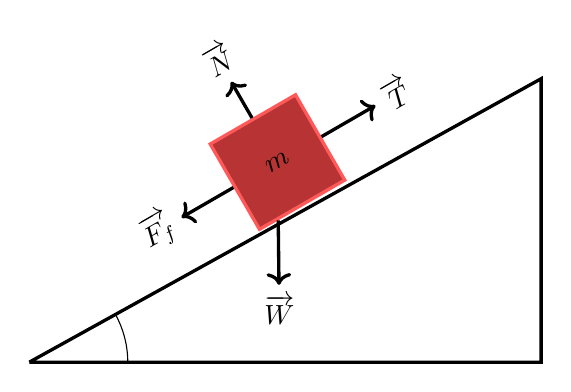
\begin{tikzpicture}[
				PhysNode/.style={rectangle, draw=red!65, fill=red!65!black!80, very thick, minimum size=1.25cm}]

			\coordinate (O) at (0,0);
			\coordinate (P1) at (6.5cm, 0cm);
			\coordinate (P2) at (6.5cm, 3.6cm);

			\draw[very thick] (O) -- (P1) -- (P2) -- (O);

			\node[PhysNode] (M) [rotate=30, xshift=4cm, yshift=0.625cm]{$m$};

			\node[very thick] (W) [below=of M, xshift=-0.3cm]{$\overrightarrow{W}$};
			\draw[very thick, ->] (M) to (W);

			\node[very thick] (N) [rotate=30, xshift=4cm, yshift=2.125cm]{$\overrightarrow{N}$};
			\draw[very thick, ->] (M) to (N);
			\node[very thick] (T) [rotate=30, xshift=5.75cm, yshift=0.625cm]{$\overrightarrow{T}$};
			\draw[very thick, ->] (M) to (T);
			\node[very thick] (Ff) [rotate=30, xshift=2.25cm, yshift=0.625cm]{$\overrightarrow{F_f}$};
			\draw[very thick, ->] (M) to (Ff);
			\tkzMarkAngle[size=1.25cm](P1,O,P2);
			\tkzLabelAngle[pos=1.5pt](P1,O,P2){\color{white}$\theta^\circ$};
		\end{tikzpicture}
		\caption{Inclined plane}
	\end{center}
\end{figure}

What is the $\theta$ such that the \emph{system} ($m_1$ and $m_2$ connected by the rope) falls with constant velocity

\begin{align*}
	\overrightarrow{F}                 & = m \overrightarrow{a}                                     \\
	w_1                                & = m_1 g                & w_2                    & = m_2 g  \\
	\phantom{=}                                                                                     \\
	\text{Resolving } m_1              & \parallel              & \text{Resolving } m_1  & \perp    \\
	T - m_1 g \sin{\theta}             & = m_1 a_1              & N - m_1 g \cos{\theta} & = 0      \\
	\phantom{=}                                                                                     \\
	\text{Resolving } m_2              &                                                            \\
	T - m_2 g                          & = m_2 a_2                                                  \\
	\phantom{=}                                                                                     \\
	\text{We can see that}                                                                          \\
	a_1                                & = a_2 = a                                                  \\
	T - m_1 g \sin{\theta}             & = m_1 a                & T - m_2 g              & = -m_2 a \\
	m_2 a + m_2 g - m_1 g \sin{\theta} & = m_1 a                                                    \\
	m_2 a + m_2 g + m_1 a              & = m_1 g \sin{\theta}                                       \\
\end{align*}

Drag caused by air resistance, we know that for low speeds $\overrightarrow{F_d} \propto - \hat{v}$

Terminal velocity: $v_\text{terminal} = v_*$ \qquad set by condition $a = 0$
%\displaystyle\int_{t_0=0}^t 
\begin{align*}
	\text{For "law speed"}                                                                                                                                                \\
	\overrightarrow{F_d}             & = -\mu_d \overrightarrow{v}                                                                                                        \\
	\phantom{=}                                                                                                                                                           \\
	mg                               & = \mu_d v_* \implies v_* = \frac{mg}{F_d}                                                                                          \\
	mg - \mu_d \underbrace{v}_{v(t)} & = m \underbrace{a}_{a(t)} = m \frac{dv}{dt}                                                                                        \\
	mg - \mu_d v                     & = m \frac{dv}{dt}                                                                                                                  \\
	dt                               & = \int_{v_0=0}^v \frac{m}{mg-\mu_d v} \, dv                                                                                        \\
	                                 & = \frac{m}{mg} \frac{1}{1 - \frac{\mu_d v}{mg}} \, dv                                                                              \\
	                                 & = \frac{1}{g} \frac{1}{1 - \frac{v}{v_*}} \, dv
	                                 & \frac{\mu_d v}{mg} = \frac{v}{\frac{mg}{\mu_d}} = \frac{v}{v_*}                                                                    \\
	                                 & = \frac{1}{g} \frac{1}{1 - \frac{v}{v_*}} \, v_* d \left(\frac{v}{v_*}\right)                                                      \\
	                                 & = \frac{1}{g} \frac{1}{1 - x} \, v_* d x                                      &  & \text{Replacing } \frac{v}{v_*} \text{ with } x \\
\end{align*}

*Not finished yet*

\section{Work}
Work done by some force $\overrightarrow{F}$
\begin{align*}
	\text{d}\overbrace{W}^\text{Work}             & = \overrightarrow{F} \cdot d \overrightarrow{s} = \overrightarrow{F} \cos{\theta} \, d \overrightarrow{s}     \\
	\phantom{=}                                                                                                                                                   \\
	W_{A \to B}                                   & = \int_A^B dW = \overbrace{\int_A^B \overrightarrow{F} \cdot d \overrightarrow{s}}^\text{Integral along path} \\
	\text{When } \overrightarrow{F} \parallel d \overrightarrow{s}                                                                                                \\
	\overrightarrow{F} \cdot d \overrightarrow{s} & = F ds                                                                                                        \\
	                                              & = F \cos{\frac{\pi}{2}} \, ds = 0                                                                             \\
	                                              & = F \cos{\pi} \, ds = -F \, ds                                                                                \\
	\phantom{=}                                                                                                                                                   \\
	[W]                                           & = [F] [L] = M \frac{L}{T^2} L                                                                                 \\
	                                              & = M \left(\frac{L}{T}\right)^2                                                                                \\
	\phantom{=}                                                                                                                                                   \\
	dW                                            & = -F_f \, ds                                                                                                  \\
	W_\text{total}                                & = \int_A^B (-F_f \, ds) = - F_f \int_A^B ds = -F_f \Bigl[s\Bigr]_\text{Start}^\text{End}                      \\
	                                              & = -F_f(s_1 - s_0)                                                                                             \\
	\phantom{=}                                                                                                                                                   \\
	dN                                            & = \overrightarrow{F_g} \cdot d \overrightarrow{s} = -mg \, dz                                                 \\
	W_{A \to B}                                   & = \int_A^B dN = -mg \Delta z
\end{align*}

\vspace{2em}

Walking shortest path $A \to B$
\begin{align*}
	W_{A \to B} & = W_{A \to B} = -F_f \Delta y
\end{align*}

Walking longer path $A \to B$ anti-clockwise
\begin{align*}
	W_{A \to B} & = W_{A \to 1} + W_{1 \to 2} + W{2 \to B}           \\
	            & = -F_f \Delta x + (F_f \Delta y) + (-F_f \Delta x) \\
	            & = -F_f (\Delta y + 2 \Delta x)
\end{align*}

Falling on path $A \to B$
\begin{align*}
	W_{A \to B} & = mg \Delta z
\end{align*}

Falling and Walking clockwise on the longer path $A \to B$
\begin{align*}
	W_{A \to B} & = W_{A \to 1} + W_{1 \to 2} + W{2 \to B} \\
	            & = 0 + mg \Delta z + 0                    \\
	            & = mg \Delta z
\end{align*}

\subsection{Example 1}
\begin{align*}
	W_{A \to B} & = E_{K_B} - E_{K_A}                                            \\
	\phantom{=}                                                                  \\
	\text{If final is conservative}                                              \\
	W_{A \to B} & \text{ is independent of path}                                 \\
	W_{A \to A} & = 0                                                            \\
	\phantom{=}                                                                  \\
	\text{Potential energy } U(A)                                                \\
	W_{A \to B} & = -(U_B - U_A)                                                 \\
	\phantom{=}                                                                  \\
	E           & = E_k + U                      &  & \text{Energy is conserved}
\end{align*}

\vspace{4em}
What happens if there is an external force?
\begin{align*}
	\overrightarrow{F}     & = \overrightarrow{F_g} + \overrightarrow{F_\text{ex}}                                                                  &  & \text{Where } \overrightarrow{F_\text{ex}} \text{ is the external force} \\
	\phantom{=}                                                                                                                                                                                                                   \\
	W_{A \to B}            & = \int_A^B \overrightarrow{F} \cdot d\overrightarrow{s}                                                                                                                                              \\
	                       & = \int_A^B \overrightarrow{F}_g \cdot d\overrightarrow{s} + \int_A^B \overrightarrow{F}_{ex} \cdot d\overrightarrow{s}                                                                               \\
	                       & = W_g + W_{ex}                                                                                                                                                                                       \\
	                       & = E_{K_B} - E_{K_B}                                                                                                                                                                                  \\
	                       & = -(U_B - U_A) + W_{cx} = E_{K_B} - E_{K_A}                                                                                                                                                          \\
	\phantom{=}                                                                                                                                                                                                                   \\
	W_{ex} + U_A + E_{K_A} & = U_B + E_{K_B}
\end{align*}

\subsection{Example 2}
\begin{align*}
	\text{Friction: } \mu                                                                                                                                                        \\
	\phantom{=}                                                                                                                                                                  \\
	v_f    & = \text{?} \qquad \text{To get to the top of ramp}                                                                    & \overrightarrow{F_f} & = - \mu N \hat{e}    \\
	v_1    & = 0                                                                                                                   & E_{k_1}              & = \frac{1}{2} mv_1^2 \\
	v_2    & = mg \, L\sin{\theta}                                                                                                 & E_{k_2}              & = 0                  \\
	w_{ex} & = \int_1^2 \overbrace{\overrightarrow{F}}^\text{\hidewidth Friction\hidewidth} \cdot \, d\overrightarrow{s}                                                         \\
	       & = \int_1^B \overrightarrow{F} \cdot \, d\overrightarrow{s} + \int_B^2 \overrightarrow{F} \cdot \, d\overrightarrow{s}                                               \\
	       & = -\mu \, mg \, d + (-\mu \, mg \, L \cos{\theta})                                                                                                                  \\
\end{align*}

\subsection{Hooke's Law}
\begin{align*}
	\text{Conservative force characterised by }                                                                             \\
	U(x)                        & = \frac{1}{2} kx^2                             &  & \text{Where } k \text{ is a constant} \\
	\phantom{=}                                                                                                             \\
	\overrightarrow{F}          & = -\frac{dU}{dx} \, \hat{e_x}                                                             \\
	                            & = - \frac{1}{2}k \cdot 2x \, \hat{e_x}                                                    \\
	                            & = -kx \, \hat{e_x}                                                                        \\
	\phantom{=}                                                                                                             \\
	\implies \overrightarrow{F} & = -k\overrightarrow{x}                         &  & \text{Hooke's Law}                    \\
	\phantom{=}                                                                                                             \\
	U_e                         & = \frac{1}{2} kx^2                             &  & \text{Elastic potential energy}       \\
	\phantom{=}                                                                                                             \\
	dW                          & = \overrightarrow{F} \cdot d\overrightarrow{x}                                            \\
	                            & = -kx \, dx
\end{align*}

\section{Linear Momentum}
\begin{align*}
	\overrightarrow{p}              & = m \overrightarrow{v}                                                                       \\
	\overrightarrow{p_\text{total}} & = \sum_k m_k \overrightarrow{v_k}                                                            \\
	                                & = m_k \sum_k \overrightarrow{v_k}                                &  & \text{If } m_k = m V_k \\
	\phantom{=}                                                                                                                    \\
	\text{For a continuous}         & \text{ distribution of mass}                                                                 \\
	dV                              & = dx^3 \qquad dm - \rho dV                                                                   \\
	\rho                            & = \text{ density } = \frac{dm}{dV} = \frac{d^3m}{dx^3}                                       \\
	\phantom{=}                                                                                                                    \\
	\overrightarrow{p}              & = \int d\overrightarrow{p}(x) = \int dm(x) \overrightarrow{v}(x)                             \\
	                                & = \int \rho(x) \overrightarrow{v}(x) dV                                                      \\
\end{align*}

\begin{align*}
	\overrightarrow{p}                                                   & = m\overrightarrow{v}                                                                                                                          \\
	\overrightarrow{F}                                                   & = m\overrightarrow{a} = \underbrace{m}_\text{\hidewidth constant\hidewidth} \frac{d\overrightarrow{v}}{dt} = \frac{d}{dt}(m\overrightarrow{v}) \\
	                                                                     & = \frac{d\overrightarrow{p}}{dt}                                                                                                               \\
	\phantom{=}                                                                                                                                                                                                           \\
	\text{If } \overrightarrow{F} = 0 \qquad                             &                                                                                                                                                \\
	\implies \frac{d\overrightarrow{p}}{dt}                              & = 0                                                                                                                                            \\
	\overrightarrow{p}                                                   & = \text{constant}                                                                                                                              \\
	\phantom{=}                                                                                                                                                                                                           \\
	dw                                                                   & = \overrightarrow{F} \cdot d\overrightarrow{s}                                                                                                 \\
	\underbrace{d\overrightarrow{J}}_\text{\hidewidth Impulse\hidewidth} & = \overrightarrow{F} dt                                                                                                                        \\
	\overrightarrow{J}                                                   & = \int_{t_1}^{t_2} \overrightarrow{F} dt
\end{align*}

\subsection{Example}
\begin{align*}
	k                               & = \text{ Label of particle}                                                                                          \\
	\phantom{=}                                                                                                                                            \\
	m                               & = 10 ~\text{kg}                                                                                                      \\
	v                               & = 2 ~\text{ms}^{-1}                                                                                                  \\
	\text{When the brick is thrown} &                                                                          & \text{After the brick hits Alberto}       \\
	p                               & = mv = 20 ~\text{kg ms}^{-1}                                             & p                                   & = 0 \\
	\phantom{=}                                                                                                                                            \\
	J                               & = \Delta p = 20 ~\text{kg ms}^{-1}                                                                                   \\
	W                               & = \Delta E = \frac{1}{2}mv_1^2 = \frac{1}{2} \times 10 \times 4 = 20 ~ J                                             \\
\end{align*}

\subsection{Centre of Mass}
\begin{align*}
	\overrightarrow{F_k}         & = m_k \overrightarrow{a_k}                                                                                                            \\
	\overrightarrow{F}           & = \sum_k m_k \overrightarrow{a_k} = \sum_k \overrightarrow{F_k}                                                                       \\
	                             & = \sum_k m_k \frac{d^2 \overrightarrow{x_k}}{dt^2}                                                                                    \\
	\phantom{=}                                                                                                                                                          \\
	\text{Centre of mass}        & \text{ of the system}                                                                                                                 \\
	\overrightarrow{F}           & = \overbrace{M}^\text{Total mass} \times \frac{d^2 \overrightarrow{R_\text{CM}}}{dt^2} = \sum_k \frac{d^2 \overrightarrow{x_k}}{dt^2} \\
	\overrightarrow{R_\text{CM}} & = \sum_k \frac{m_k}{M} \overrightarrow{x_k}
\end{align*}

\subsection{Collisions}
\begin{itemize}
	\item{Totally \underline{inelastic} colliion --- After the collision the bodies stick}
	\item{Totally \underline{elastic} colliion --- After the collision the bodies travel in opposite directions}
\end{itemize}

\begin{align*}
	P_A             & = M u_1 + m u_2                               & P_B & = M v_1 + m v_2 \\
	                &                                               &     & = (M + m) v     \\
	\phantom{=}                                                                             \\
	P_A             & = P_B                                                                 \\
	M u_1 + m u_2   & = (M + m) v                                                           \\
	v               & = \frac{M u_1 + m u_2}{M + m}                                         \\
	\phantom{=}                                                                             \\
	\text{Assume } \qquad u_1 > 0 \quad u_2 = 0 \quad M >> m                                \\
	v               & = \frac{M u_1}{M + m}                                                 \\
	                & = \frac{M}{M + m} \, u_1                                              \\
	\phantom{=}                                                                             \\
	\frac{m}{M}     & = \varepsilon \ll 1                                                   \\
	\phantom{=}                                                                             \\
	\frac{M}{M + m} & = \frac{M}{M(1 + \frac{m}{M})}                                        \\
	                & = \frac{1}{1 + \varepsilon}                                           \\
	                & = (1 + \varepsilon)^{-1}                                              \\
	                & = 1 - \epsilon + O(\varepsilon^2)                                     \\
	\phantom{=}                                                                             \\
	v               & = (1 - \varepsilon + O(\varepsilon^2)) \, u_1
\end{align*}

Now imagine the truck is at rest

\begin{align*}
	v      & = \frac{m u_2}{M + m}                                                   \\
	       & = \frac{m}{M + m} \, u_2                                                \\
	\phantom{=}                                                                      \\
	\delta & \ll 1                                            &  & \text{Mass ratio} \\
	\delta & = \varepsilon = \nicefrac{m}{M} \ll 1                                   \\
	\phantom{=}                                                                      \\
	v      & = \frac{m}{M + m} \, u_2                                                \\
	       & = \frac{\nicefrac{m}{M}}{\frac{M + m}{M}} \, u_2                        \\
	       & = \frac{m}{1 + \nicefrac{m}{M}} \, u_2                                  \\
\end{align*}
*Not finished*

\subsection{Totally elastic collisions}
\begin{align*}
	\overrightarrow{P} =                          & \text{ const}                                                                                     \\
	\overrightarrow{E_k} =                        & \text{ const}                                                                                     \\
	\phantom{=}                                                                                                                                       \\
	m_1 u_1 + m_2 u_2                             & = m_1 v_1 + m_2 v_2                                                                               \\
	\frac{1}{2} m_1 v_1^2 + \frac{1}{2} m_2 u_2^2 & = \frac{1}{2} m_1 v_1^2 \frac{1}{2} m_2 v_2                                                       \\
	m_1 u_1^2 + m_2 u_2^2                         & = m_1 v_1^2 m_2 v_2                                                                               \\
	\implies m_1(u_1^2 - v_1^2)                   & = m_2(v_2^2 - u_2^2)                                                                              \\
	m_1(u_1 - v_1)(u_1 + v_1)                     & = m_2(v_2 - u_2)(v_2 + u_2)                                                                       \\
	\implies u_1 + v_1                            & = v_2 + u_2
	                                              &                                             & \text{Using } m_1 u_1 + m_2 u_2 = m_1 v_1 + m_2 v_2 \\
	\phantom{=}                                                                                                                                       \\
	v_1 - v_2                                     & = u_2 - u_1 = -(u_1 - u_2)
\end{align*}

Using conservation of energy
\begin{align*}
	E_k                      & = \frac{1}{2} M u_1^2 = \frac{1}{2} M v_1^2 + \frac{1}{2} m v_2^2                                           \\
	\overrightarrow{p}       & = p_x + p_y                                                                                                 \\
	p_x \text{:} \qquad Mu_1 & = M v_1 \cos{\alpha} + m v_2 \cos{\beta}
	                         & p_y \text{:} \qquad 0                                             & = M v_1 \sin{\alpha} - mv_2 \cos{\beta}
\end{align*}

\subsection{Angular momentum}
\begin{align*}
	\overrightarrow{L}              & = \overrightarrow{R} \times \overrightarrow{P} = \overrightarrow{R} \times (m \overrightarrow{v})                                       \\
	\left|\overrightarrow{L}\right| & = \overrightarrow{R} \, p \sin{\theta}                                                                                                  \\
	\phantom{=}                                                                                                                                                               \\
	\frac{d\overrightarrow{L}}{dt}  & = \frac{d}{dt}\left(\overrightarrow{R} \times \overrightarrow{p}\right)                                                                 \\
	                                & = \frac{d}{dt}\left(\overrightarrow{R} \times m \overrightarrow{v}\right)                                                               \\
	                                & = m \, \frac{d}{dt}\left(\overrightarrow{R} \times \overrightarrow{v}\right)                                                            \\
	                                & = m \, \left[\frac{d\overrightarrow{R}}{dt} \times \overrightarrow{v} + \overrightarrow{R} \times \frac{d\overrightarrow{v}}{dt}\right] \\
	                                & = m \left(\overrightarrow{v} \times \overrightarrow{v} + \overrightarrow{R} \times \overrightarrow{R}\right)                            \\
\end{align*}

\section{Gravitation}
*This is in book*

\section{Potential Energy}
\begin{align*}
	\overrightarrow{F} &= - G\frac{m_1m_2}{R^2} \hat{R}\\
	&= -\overrightarrow{\bigtriangledown} U \qquad \sim \qquad \overrightarrow{F} = -\frac{dU}{dR}\hat{R}\\
\end{align*}
\end{document}